%%%%%%%%%%% Aquí va la solución al problema 1.
\newpage
\textbf{\textcolor{MidnightBlue}{1.}} Considera la siguiente variante del algoritmo de consenso con terminación temprana.
Contesta lo siguiente:
\begin{enumerate}
    \item Demuestra que el algoritmo 1 soluciona el problema del consenso, tolerando $f < n$ fallas de tipo paro, donde $n$ es el número de procesos en el sistema.
    
    Por demostrar:
    \begin{itemize}
        \item Terminación
        
        El algoritmo no tiene una clara condición de salida. La linea 6 se ejecutara indefinidamente, a menos que exista una en la linea 9 cuando se ejecuta \textit{decide max(vista)}.
        
        \item Validez
        
        El valor de \textit{prop = vista} fue propuesto por algún proceso en cada ronda.

        \item Acuerdo. 
        No queda claro si el algoritmo termina, sin embargo:
        Veamos una ejecución cuando $f=0$:
        Al inicio de la ejecución $r=0$, la \textit{flag = false}, 
        envía $<prop,false>$, luego $r=1$, 
        $vista = prop, prop_1$, luego  
        $rec[1]= 1+1$ y no se modifica \textit{flag} 
        hasta que $rec[1-1]==rec[1]$, 
        en esta ronda no se modifica \textit{flag}

        
        Cuando $r=2$, 
        $send(<prop_2,false>)$ a todos
        \textit{vista = \{$prop,prop_1,prop_2$\}}
        $rec[2]=1+1$

        $rec[2-1]==rec[2] \rightarrow rec[1]==rec[2]$, en esta ronda se modifica $flag=true$

        
        Cuando $r=3$, 
        $send(<prop_2,true>)$ a todos
        \textit{decide max(vista)}
        \textit{vista = \{$prop,prop_1,prop_2,prop_3$\}}
        \textit{ dec = true}
        $rec[3]=1+3$
        $rec[3-1]==rec[3] \rightarrow rec[2]==rec[3]$, en esta ronda no se modifica $flag=true$


        Cuando $r=4$, 
        $send(<prop_3,true>)$ a todos
        \textit{decide max(vista)}
        \textit{vista = \{$prop,prop_1,prop_2,prop_3,prop_4$\}}
        \textit{dec = true}
        $rec[4]=1+3$

        $rec[4-1]==rec[4] \rightarrow rec[3]==rec[4]$, en esta ronda no se modifica $flag=true$

        Si algún proceso tuviera una falla de tipo paro, el valor de vista sería diferente y si al menos una flag de la ronda anterior es verdadera entonces llega a un acuerdo con los valores de vista.
        Por lo tanto en cada dos rondas a partir de la tercera, todos los proceso (vivos) acuerdan el mismo valor.
    \end{itemize}
    

    \item ¿Es cierto que los procesos correcto terminan en a lo más $max(t +2, f +1)$ rondas en el algoritmo 1? Argumenta tu respuesta. Recuerda que $t \leq f$ es el número de fallas que realmente ocurren en una ejecución dada.
    \item 
    t es el número de fallas que realmente ocurren en una ejecución$+1$.
    f es el número de fallas de tipo paro$+2$.
    
    \item Haz un análisis del número máximo de mensajes que se envían en una ejecución del algoritmo 1. Tu cota debe estar en función de $n$ y $f$.
\end{enumerate}

\begin{figure}
    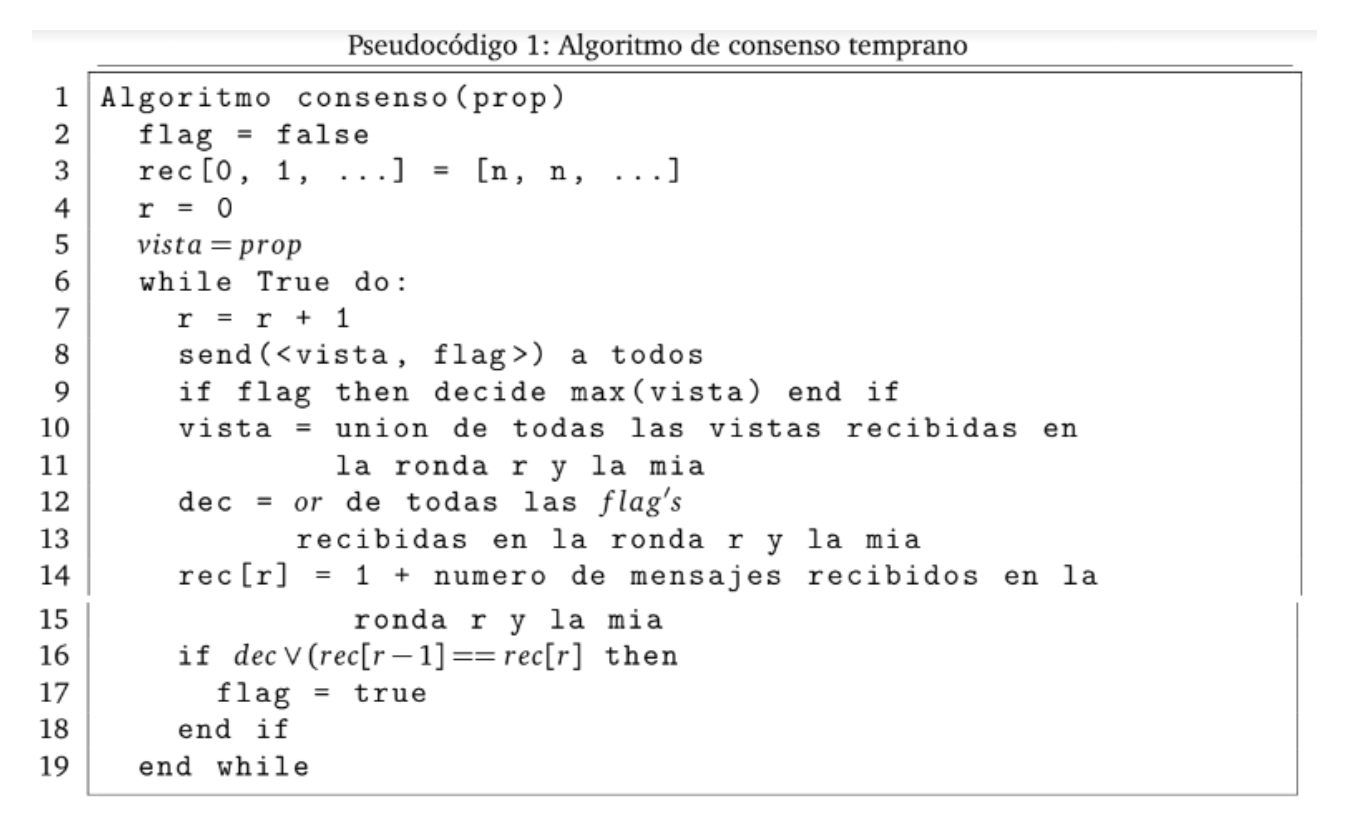
\includegraphics[width=\textwidth]{consensoTemprano.png}
\end{figure}